\documentclass[14pt]{article}

\usepackage[letterpaper,bindingoffset=0.2in,%
            left=1in,right=1in,top=1in,bottom=1in,%
            footskip=.25in]{geometry}
\usepackage[english]{babel}
\usepackage[utf8x]{inputenc}
\usepackage{amsmath}
\usepackage{amssymb}
\usepackage{amsthm}
\usepackage{graphicx}
\usepackage[makeroom]{cancel}
\usepackage{booktabs}
\usepackage{enumitem}
\usepackage{tabularx}
\usepackage{xcolor}
\usepackage{hyperref}
\usepackage{tikz}
\usepackage{pgfplots}
\pgfplotsset{compat=1.11}
\usepackage{systeme}
\usepackage{calc}
\usepackage{caption}
\usepackage{subcaption}
\usepackage{multicol}

\usetikzlibrary{calc}
\usetikzlibrary{positioning}
\usetikzlibrary{arrows,decorations.markings}

\graphicspath{ {./images/} }


% DOCUMENT STARTS HERE

\begin{document}

\title{Analysis H Project: \\ \textbf{3D Graphics Generation with Matrices}}
\author{Mihir Rao}
\maketitle

\begin{center}
	\vspace{3em}
	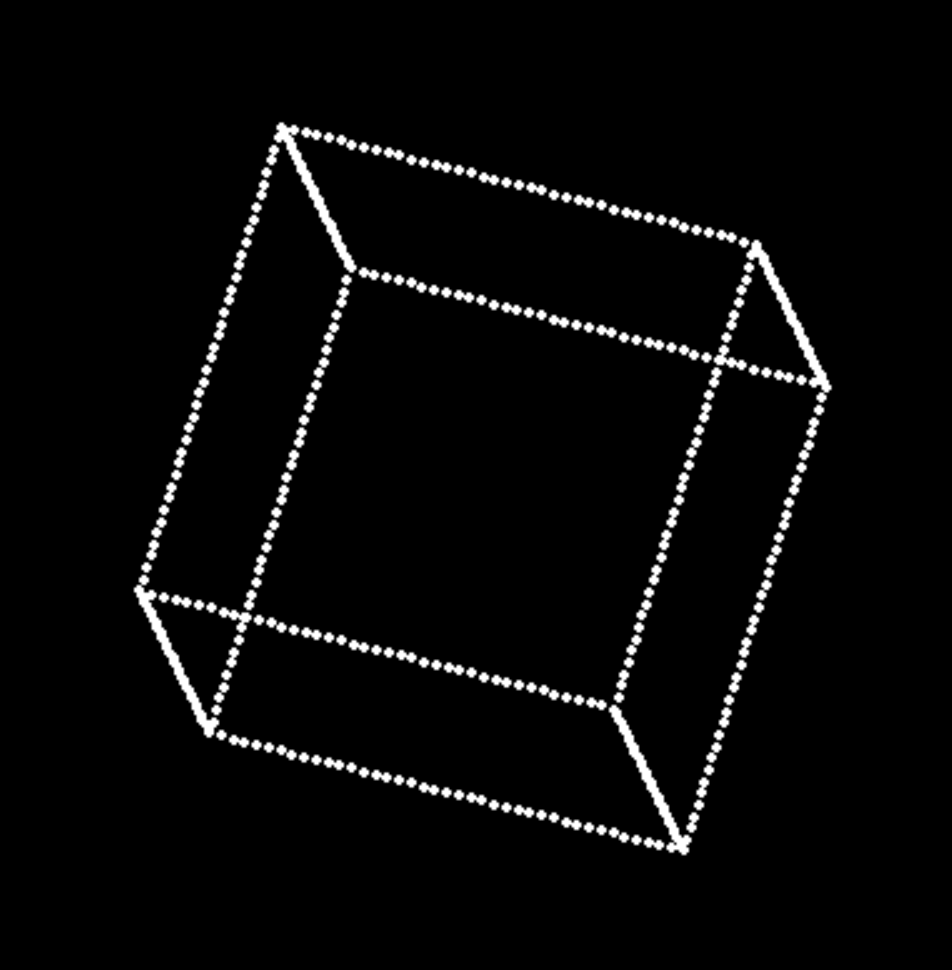
\includegraphics[scale=0.8]{titleImg}
	\vspace{3em}
\end{center}

\section*{Overview}

Overview stuff

\newpage

\section*{Introduction}

Introduction stuff.

\section*{The Math}

Math stuff.

\end{document}